\section{Main Results \label{sec:main}}

For a given family of dictionaries $F_{N, d} \in \R^{N \times d},$ consider the problem of recovering a random $k$-element subset $X$ from a $d$-dimensional superposition code. Let
$$
b(d, k, N; \tau), \quad b(d, k, N; \text{top-}k)
$$
denote the respective failure probabilities for threshold decoding at level $\tau$ and for top-$k$ decoding.\footnote{The letter $b$ is a mnemonic for the ``bad event.''} Naturally we have $b(d, k, N; \text{top-}k) \le b(d, k, N; \tau),$ since if a given code $Y$ is accurately decoded by threshold decoding at any level, it is also decoded by top-$k.$

Our first result provides an asymptotic constraint on the dimension $d$ required for either of these values to be converge to $0$ for large $N.$

\begin{proposition} \label{prop:necessary-cond}
    Let $\epsilon > 0$ be arbitrary. Over the regime
    $$
    d \le (1 - \epsilon) 2 k \ln N, \quad 2 \le k < N/2,
    $$
    for random spherical dictionaries it holds that
    $$
    \lim_{N \to \infty} b(d, k, N; \text{top-$k$}) = 1.
    $$
\end{proposition}

This proposition is stated for spherical dictionaries, but similar results can naturally be proven for other kinds of random dictionaries. Also note that this result agrees with the informal derivation based on a Shannon limit that we described in the previous section. In fact, it is likely possible to prove \Cref{prop:necessary-cond} by a refinement of such an information-theoretic argument. However, our proof (in \Cref{appendix:proofs}) simply uses concentration inequalities to provide adequate lower bounds on the quantity $b(d, k, N; \text{top-$k$)}.$

Now, in a regime when $k \ge \epsilon N$ for some $\epsilon > 0$, the entropy of the variable $X$ being transmitted is
$$
H = \ln \binom{N}{k} \le k \ln \left( \frac {eN} k \right) = O(N).
$$
However, \Cref{prop:necessary-cond} shows that we need at least $d = \Omega(k \ln N) = \Omega(N \ln N)$ dimensions for top-$k$ to read a superposition code, which is asymptotically larger. In a regime $k \ge \epsilon N,$ we can informally say that the amount of information that top-$k$ can read from each dimension of the code converges to $0.$

Is it natural to ask whether a one-step decoder can be ``information-efficient'' in some sparser regime. By our discussion, we would need $H / (k \ln N)$ to be bounded below. Since
$$
\frac{H} {k \ln N} = \frac{k \ln N - k \ln k + O(k)}{k \ln N} = 1 - \frac{\ln k} {\ln N} + O\left(\frac 1 {\ln N}\right),
$$
we conclude that one-step decoders can only be information-efficient in a regime where $\ln k / \ln N$ is bounded strictly below 1.

This calculation motives us to introduce a parameter $\eta = \ln k / \ln N,$ which we call the sparsity exponent. In compressive sensing, when $k \le N^\eta$ we say we are in a regime of \textit{sublinear sparsity}. Our next result gives a sufficient condition for threshold decoding to succeed asymptotically in such a regime.

\begin{proposition}\label{prop:sufficient-cond}
    For $\eta \in (0, 1],$ let $k \le N^\eta.$ Then for any $\epsilon > 0,$ over the regime
	$$
	d \ge (1 + \epsilon) 2(1 + \sqrt \eta)^2 k \ln N,
	$$
	for Rademacher dictionaries it holds that
	$$
	\lim_{N \to \infty} b(d, k, N; \tau(\eta)) = 0,
	$$
	where $\tau(\eta) = (1 + \sqrt \eta)^{-1}.$
\end{proposition}

Note that the value of $\tau$ is connected (but not identical) to the MAP threshold we derived in \Cref{sec:codes}. It is a simple corollary of \Cref{prop:sufficient-cond} that MAP thresholding has the same asymptotic guarantee. See \Cref{appendix:proofs} for proofs of \Cref{prop:necessary-cond} and \Cref{prop:sufficient-cond}, as well as a discussion of this connection.

Putting $\eta = 1,$ the condition $k \le N^\eta$ becomes vacuous and overall we conclude that $d \ge (1 + \epsilon) 8 k \ln N$ dimensions are enough for threshold decoding to succeed with threshold $\tau = 1/2$ for any $k$ as $N \to \infty.$ Meanwhile, as $\eta$ goes to $0$ the factor $2 (1 + \sqrt \eta)^2$ converges to $2,$ which matches \Cref{prop:necessary-cond}.

\begin{figure}[!htbp]
\begin{subfigure}[b]{\textwidth}
\centering
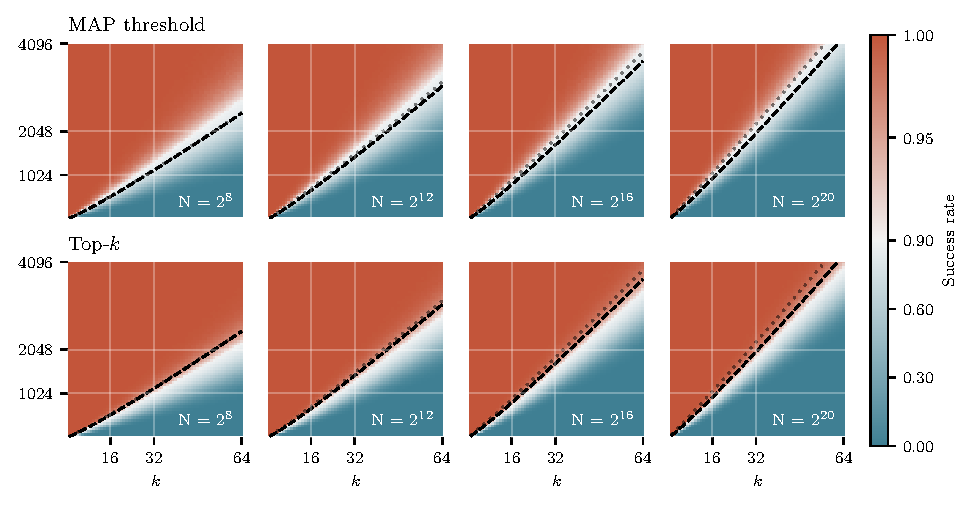
\includegraphics[width=0.85\textwidth]{../figures/k_sweep}
\caption{Empirical performance of MAP thresholding and top-$k$ thresholding at decoding a $k$-element subset of $[N]$ from a $d$-dimensional superposition code using a random spherical dictionary. The dashed line shows the critical value $d = 2 (1 + \sqrt{\eta})^2 k \ln N$ predicted for threshold decoding by \Cref{prop:sufficient-cond}.}
\label{fig:k-sweep}
\end{subfigure}
\vspace{0.2em}
\begin{subfigure}[b]{\textwidth}
\centering
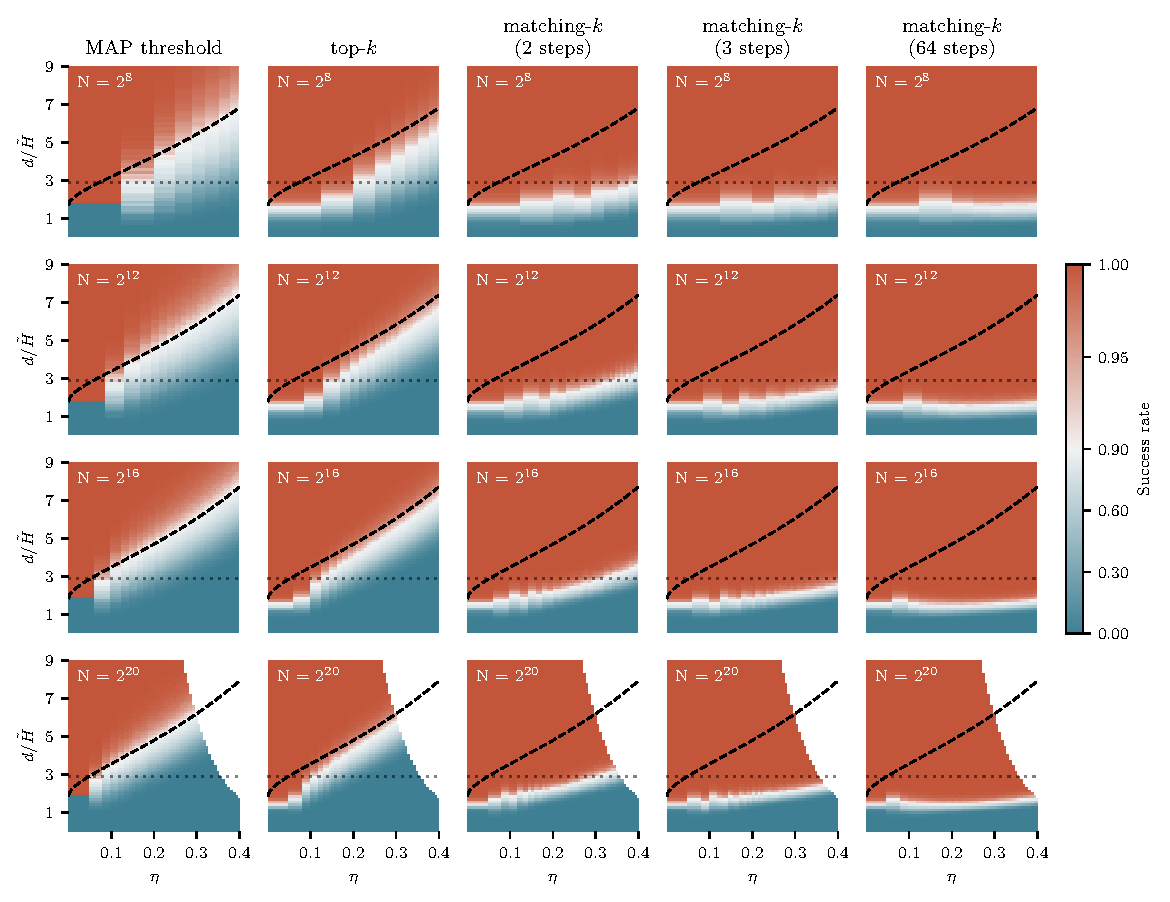
\includegraphics[width=1\textwidth]{../figures/eta_sweep}
\caption{\textbf{How many dimensions do we need to store one bit of information?} We graph empirical performance of MAP thresholding, top-$k$, and GMP at exactly decoding a superposition code as a function of approximate inverse bitrate $d / \tilde H_2 = d / (k \log_2(e N/k))$ and the sparsity exponent $\eta = \ln k / \ln N.$ The bold line shows the critical value $d = 2 (1 + \sqrt \eta)^2 k \ln N$ predicted by \Cref{prop:sufficient-cond} and thin line shows the limit described in \Cref{prop:information-statement} as $N \to \infty.$ In all cases, we use a dictionary of random spherical codewords.}
\label{fig:eta-sweep}
\end{subfigure}
\end{figure}

\Cref{fig:k-sweep} shows how the critical value $d_\text{crit} = 2 (1 + \sqrt \eta)^2 k \ln N$ appearing in the statement of \Cref{prop:sufficient-cond} compares with empirical performance of MAP thresholding and top-$k$ for finite values of $N$ and $k.$ For $k < 64$ and values of $N$ ranging over several orders of magnitude, the value $d_\text{crit}$ can be used to reliably predict the performance of both decoding methods.

Now we return to the information-theoretic point of view. Using the fact that
$$
\frac H {k \ln N} = 1 - \eta + O\left ( \frac 1 {\ln N} \right),
$$
we can restate \Cref{prop:sufficient-cond} in the following way, which is asymptotically equivalent for $\eta < 1.$

\begin{corollary} \label{prop:information-statement}
For $\eta \in (0, 1),$ let $k \le N^\eta$ and let $H = \ln \binom N k.$ Then for any $\epsilon,$ over the regime
$$
\frac{d}{H} \ge (1 + \epsilon) \frac {2 (1 + \sqrt \eta)} {1 - \sqrt \eta}
$$
we have the same conclusion as \Cref{prop:sufficient-cond}.
\end{corollary}

When $\eta < 1/2,$ note that entropy can be approximated more exactly by
$$
\tilde H = k \ln (e N / k) = \ln \binom N k + o(1),
$$
(see \Cref{appendix:binomial}) and as a consequence
$$
\frac H {k \ln N} = 1 - \eta + \frac 1 {\ln N} + O\left ( \frac 1 {k \ln N}\right).
$$
Therefore, if we take the expression $d_\text{crit} = 2 (1 + \sqrt \eta)^2 k \ln N$ in \Cref{prop:sufficient-cond} as a ``rule of thumb'' for finite values of $(k, N),$ the ratio $d_\text{crit}/H$ is closer to
$$
\frac{d_\text{crit}}{\tilde H} = \frac{2 (1 + \sqrt \eta)^2}{1 - \eta + 1 / \ln N}.
$$
Although this is not proven

The two left-most columns of \Cref{fig:eta-sweep} show the critical value of $d$ predicted by \Cref{prop:sufficient-cond} in terms of the inverse bitrate $d/\tilde H_2$ as a function of $\eta,$ compared against the empirical performance of MAP thresholding and top-$k$. (Here $\tilde H_2 = \tilde H / \ln 2 \approx \log_2 \binom N k.$) Empirical results on the bottom row are truncated at the point that would require a dictionary with dimensions larger than $2^{20} \times 4096.$ Over the range $N = 2^8, \dots, 2^{20}$ and $\eta \in (0, 0.4),$ these predictions track the performance of MAP thresholding and top-$k.$

For the values $N = 2^{20}$ and $k = 64$ we referenced from \citet{gao_scaling_2024}, we have $\eta = \ln k / \ln N = 0.3,$ and the predicted critical value of $d/H$ is roughly
$$
\frac{2 \left(1 + \sqrt{0.3}\right)}{1 - 0.3 + 6 \ln 10} \approx 6.2
$$
dimensions per nat, or around $4.3$ dimensions per bit. Indeed, we find for all $N$ that when $\eta = 0.3,$ more than $4$ dimensions per bit are needed for MAP thresholding to work reliably. The performance of top-$k$ is noticeably better but limited in a similar way.

On the other hand, even with only $T = 3$ steps, generalized matching pursuit (GMP) succeeds reliably with $d/\tilde H_2 > 2$ over the range $\eta \in (0, 0.4).$ In the case $N = 2^{20}$ and $k = 64,$ three-step GMP decreases the required dimensions by a factor of more than $2.$ Increasing the step parameter further shows noticeable but diminishing returns.
